\documentclass{beamer}
\usepackage{tikz}
\usepackage{verbatim}

\usetikzlibrary{positioning}
\usetikzlibrary{shapes.geometric, arrows}
\usetikzlibrary{tikzmark}

% theme options
\usetheme{default}
\usecolortheme{crane}

\definecolor{ui_brave_gold}{cmyk}{0, 0.105, 1, 0}
\definecolor{ui_silver}{cmyk}{0,0,0, 0.196}
\definecolor{ui_black}{rgb}{0,0,0}


% add logo to slides
\logo{
    \includegraphics[width=2.5cm]{./UI_Dept_CDA_Computer_Sci_horizontal_4c.png}
}

\setbeamercolor*{structure}{bg=ui_brave_gold,fg=ui_black}

\setbeamercolor*{palette primary}{use=structure,fg=white,bg=structure.fg}
\setbeamercolor*{palette secondary}{use=structure,fg=white,bg=structure.fg!75}
\setbeamercolor*{palette tertiary}{use=structure,fg=white,bg=structure.fg!50!black}
\setbeamercolor*{palette quaternary}{fg=white,bg=black}

\setbeamercolor{section in toc}{fg=black,bg=white}
\setbeamercolor{alerted text}{use=structure,fg=structure.fg!50!black!80!black}

\setbeamercolor{titlelike}{parent=palette primary,fg=structure.fg!50!black}
\setbeamercolor{frametitle}{bg=ui_black,fg=ui_brave_gold}

\setbeamercolor*{titlelike}{parent=palette primary}

\begin{document}
\pgfdeclarehorizontalshading[ui_silver, ui_black]{ui_title_banner}{\pagewidth}{ui_silver, ui_black, ui_silver}

% "plain" arg creates empty slide

{
\setbeamercolor{background canvas}{bg=ui_black}
\begin{frame}[plain]


    \begin{tikzpicture}[remember picture, overlay]
        % TITLE SLIDE LOGO
        \node[above right, inner sep=0pt] at (current page.south west)
        {
            %\includegraphics[width=100px]{./UI_Dept_CDA_Computer_Sci_horizontal_4c.png}
        };

        \node
        [
            above=0.5cm,
            align=center,
            %fill=ui_brave_gold,
            %right color=ui_silver,
            %middle color=ui_black,
            %left color=ui_silver,
            top color = ui_black,
            bottom color = ui_brave_gold!70!ui_black,
            %shading=ui_title_banner,
            %rounded corners,
            inner xsep=15pt,
            inner ysep=10pt, 
            minimum width=\paperwidth,
            text width=0.9\textwidth
        ] (title) at (current page.center)
        {
            \LARGE \textcolor{ui_brave_gold}{A Vandalized Introduction to ROS2}\\[5pt]
            \small \textcolor{ui_brave_gold!20}{written by barbarians for barbarians!}
        };

        % Author 
        \node[below=0.5cm] (author) at (title.south){\textcolor{ui_silver}{Garrett Wells}};
        % Date
        \node[below=0.5cm] (date) at (author.south){\textcolor{ui_silver}{\large \today}};
        % Logo
        \node
        [
            below right =0.25cm and 0.5cm
        ] at (current page.north west)
        {
            \includegraphics[width=3.5cm]{./UI_Dept_CDA_Computer_Sci_horizontal_4c.png}
        };

    \end{tikzpicture}

\end{frame}
}

\begin{frame}{Table of Contents}
    \tableofcontents
\end{frame}

\section{What is ROS2?}
\begin{frame}{\textit{What is ROS2?}}

    \begin{block}{From the Horse's Mouth}
        \textit{\textbf{The Robot Operating System (ROS) is a set of software libraries and tools for building robot applications.}} From drivers and state-of-the-art algorithms to powerful developer tools, ROS has the open source tools you need for your next robotics project.
    \end{block}

    \only<2>{
        \begin{itemize}
            \item Open source software! Whoopee!
            \item Tries to abstract robots and sensors as \textbf{producers} and \textbf{consumers} of data
            \item Solves \textit{almost} as many problems as it creates
        \end{itemize}
        \begin{tikzpicture}{}
            \node
            [
                above right
            ] at (current page.north east)
            {
                \includegraphics[width=0.1\textwidth]{./noetic-background.png}
            };
        \end{tikzpicture}
    }
    \only<1>{\centering\includegraphics[width=0.4\textwidth]{./ros_features.png}}

\end{frame}

\subsection{Abstracting Machines as Data}
\begin{frame}[fragile]{\textit{Abstracting Machines as Streams of Data}} 
    \begin{tikzpicture}{}
        \node
        [
            anchor=east
        ] (bots)
        {
            \includegraphics[width=0.25\textwidth]{./TurtleBotsFacing.jpg}
        };

        \node
        [
           anchor=west
        ] (ros_arch)
        {
            \includegraphics[width=0.6\textwidth]{./ros_graph_example-1773129841.png}
        };

        \node
        [
            rectangle,
            fill=gray!20,
            outer sep=10,
            rounded corners
        ] (wesee) at (bots.north)
        {what we see};

        \node
        [
            rectangle,
            fill=gray!20,
            rounded corners,
        ] (rossee) at (ros_arch.north)
        {what ros sees};

    \end{tikzpicture}
    \vspace{0.1cm}\\
    \only<2>{
        \begin{block}{What is a Node?}
            A node is a participant in the ROS 2 graph, which uses a client library to communicate with other nodes. Nodes can communicate with other nodes within the same process, in a different process, or on a different machine. Nodes are typically the unit of computation in a ROS graph; each node should do one logical thing.
        \end{block}
        \href{https://docs.ros.org/en/iron/Concepts.html}{\beamerbutton{ROS Concepts Documentation Link}}
    }
    \only<3>{
        \textbf{Nodes in Example:} camera driver, blob finder, target follower, motor driver
        \vspace{0.5cm} \\
        \centering
        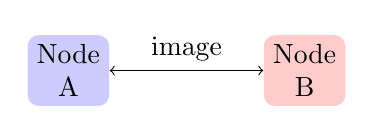
\begin{tikzpicture}{}
            \node (A) at (0,-1) [align=center, rectangle, rounded corners, fill=blue!20]{Node\\A};
            \node (B) at (3cm,-1) [align=center, rectangle, rounded corners, fill=red!20]{Node\\B};
            \draw[<->] (A) -- (B) node [pos=0.5, above]{image};

        \end{tikzpicture}
    }

    \only<4->{
        \begin{itemize}
                \only<4-5>{
                    \item \textbf{camera driver : \tikzmarknode[draw, inner sep=2pt, rounded corners, fill=green!20]{A}{producer}} interfaces with hardware to capture image, then publishes to topic (\textbf{image})
                }
                \only<5>{ 
                    \item \textbf{motor driver : \tikzmarknode[draw, inner sep=2pt, fill=red!20, rounded corners]{B}{consumer}} consumes data from topic (\textbf{steering direction}) and then interfaces with motors to move forward
                }
                \only<6>{
                    \item ROS2 refers to nodes that are \textbf{producers} as \textbf{publishers}
                    \item can publish as needed or at a frequency, ex. 10Hz
                    \item topics are identified with a path, ex. \textit{/robot/odom}
                }
                \only<7>{
                    \item ROS2 refers to nodes that are \textbf{consumers} as \textbf{subscribers}
                    \item subscribers use path to subscribe to a topic
                }
                
        \end{itemize}
    }

\end{frame}


\subsection{The ROS2 Stack}
\begin{frame}{\textit{The ROS2 Stack}}
    \only<1>{
        \includegraphics[width=\textwidth]{./ros2\_stack.png}
    }
    \only<2>{
        \includegraphics[width=\textwidth]{./ros1vs2\_stack.png}
    }
\end{frame}

\section{ROS2 Concepts}
{
\setbeamercolor{background canvas}{bg=ui_black}
\begin{frame}[plain]{}
    \begin{tikzpicture}[remember picture, overlay]
        \node
        [
            above=0.5cm,
            align=center,
            %fill=ui_brave_gold,
            %right color=ui_silver,
            %middle color=ui_black,
            %left color=ui_silver,
            fill = ui_brave_gold,
            %shading=ui_title_banner,
            rounded corners,
            inner xsep=15pt,
            inner ysep=10pt, 
            minimum width=0.8\paperwidth,
            text width=0.9\textwidth
        ] (title) at (current page.center)
        {
            \LARGE \textcolor{black}{\textbf{ROS2 Concepts}
        }};
        \node[below=0.5cm] (subtitle) at (title.south){\textcolor{white}{Topics, Actions, Servers, Workspaces, and Client Libraries}};

    \end{tikzpicture}

\end{frame}
}

\subsection{Topics}
\begin{frame}{\textit{Topics}}
    \begin{itemize}
        \item topics created by publishing/subscribing nodes
        \item available to all devices on network
        \item topics are forward slash separated paths
        \item messages are strongly typed structs
        \item messages are anonymous by default
    \end{itemize}

    \href{https://docs.ros.org/en/iron/Tutorials/Beginner-CLI-Tools/Understanding-ROS2-Topics/Understanding-ROS2-Topics.html\#background}{\beamerbutton{ROS2 Topics Example Link}}
\end{frame}

\subsubsection{Topic Illustration}
\begin{frame}[fragile]{\textit{Topic Illustration: Using A Standard ROS2 Topic}}
    \textbf{So what does a topic message consist of?} \\
    \vspace{0.5cm} 
    \textbf{topic:} \verb|/odom [nav_msgs/msg/Odometry]| \\
    \textbf{topic message:} 
    \begingroup
    \fontsize{6pt}{12pt}\selectfont
    \begin{verbatim}
# This represents an estimate of a position and velocity in free space.  
# The pose in this message should be specified in the coordinate frame given by header.frame_id.
# The twist in this message should be specified in the coordinate frame given by the child_frame_id
Header header
string child_frame_id
geometry_msgs/PoseWithCovariance pose
geometry_msgs/TwistWithCovariance twist
    \end{verbatim}
    \endgroup

\end{frame}

\subsection{Actions}
\begin{frame}{\textit{Actions}}
    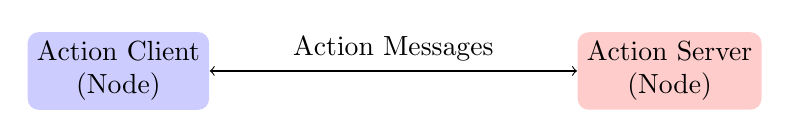
\begin{tikzpicture}{}
        \node
        [
            align=center,
            rectangle,
            rounded corners,
            fill=blue!20
        ] (A) at (0, 0) {Action Client\\(Node)};
        \node
        [
            align=center,
            rectangle,
            rounded corners,
            fill=red!20
        ] (B) at (7cm, 0){Action Server\\(Node)};
        \draw[<->] (A) -- (B) node [pos=0.5, above]{Action Messages};
    \end{tikzpicture}
    \vspace{0.5cm}
    \begin{block}{Action}
        Consists of three parts:
        \begin{itemize}
            \item Goal: \textit{a message containing what you wish to be done}
            \item Feedback: \textit{a message from the action server}
            \item Result: \textit{the success/failure message from server}
        \end{itemize}
    \end{block}
    \vspace{0.5cm}
    Check out the example tutorial and documentation:
    \href{https://docs.ros.org/en/iron/Tutorials/Beginner-CLI-Tools/Understanding-ROS2-Actions/Understanding-ROS2-Actions.html}{\beamerbutton{ROS2 Actions Documentation Link}}
\end{frame}

\subsection{Services}
\begin{frame}{\textit{Services}}
    {\Huge Services are call and response versions of topics}
    \begin{block}{Services}
        While topics allow nodes to subscribe to data streams and get continual updates, services \textbf{only provide data when they are specifically called by a client}.
    \end{block}

    Used to request that computation heavy tasks be completed by another node. (Google, tell me the 10th digit of Pi!)

    \begin{itemize}
        \item consist of a \textit{request} and a \textit{response}
    \end{itemize}

    \href{https://docs.ros.org/en/iron/Tutorials/Beginner-CLI-Tools/Understanding-ROS2-Services/Understanding-ROS2-Services.html\#background}{\beamerbutton{Services GIF Link}}
\end{frame}

\subsection{Client Libraries}
\begin{frame}{\textit{Client Libraries}}
    {\Huge Client Libraries provide access to the ROS2 API including:}
    \begin{itemize}
        \item Node functions
        \item topic pub/sub functions
        \item actions
        \item services
    \end{itemize}

    \textit{available for C++, Python, and more!}

    \href{https://docs.ros.org/en/humble/Concepts/Basic/About-Client-Libraries.html?highlight=rclpy}{\beamerbutton{ROS Client Libraries Link}}
\end{frame}

\begin{frame}[fragile]{RCL Example}
    \begin{verbatim}
node = rclpy.create_node('minimal_publisher')
publisher = node.create_publisher(String, 'topic', 10)
    \end{verbatim}

    \href{https://github.com/ros2/examples/tree/rolling}{\beamerbutton{GitHub RCL Examples Link}}
\end{frame}

\begin{frame}[fragile]{RCL Inheritance}
    \begingroup
    \fontsize{8pt}{10pt}\selectfont
    \begin{verbatim}
import rclpy
from rclpy.node import Node

from std_msgs.msg import String


class MinimalPublisher(Node):

    def __init__(self):
        super().__init__('minimal_publisher')
        self.publisher_ = self.create_publisher(String, 'topic', 10)
        timer_period = 0.5  # seconds
        self.timer = self.create_timer(timer_period, self.timer_callback)
        self.i = 0
    \end{verbatim}
    \endgroup

    \href{https://github.com/ros2/examples/blob/rolling/rclpy/topics/minimal_publisher/examples_rclpy_minimal_publisher/publisher_member_function.py}{\beamerbutton{Example Source Code}}
\end{frame}

\subsection{Workspaces}
\begin{frame}{\textit{Workspaces}}
    \only<1>{
        \begin{block}{Workspaces}
            \textbf{A workspace is a directory containing ROS 2 packages.} Before using ROS 2, it’s necessary to \textbf{source} your ROS 2 installation workspace in the terminal you plan to work in. This makes ROS 2’s packages available for you to use in that terminal.
        \end{block}

        \begin{block}{Package}
            A package is an organizational unit (directory) for your ROS 2 code. Packages may contain metadata and scripts that help run and build the package.
        \end{block}

    }
\end{frame}

\begin{frame}[fragile]{Example Workspace Structure: Pre\--Build}

    \begingroup
    \fontsize{10pt}{11pt}\selectfont
    \begin{verbatim}
workspace_folder/
    src/
      cpp_package_1/
          CMakeLists.txt
          include/cpp_package_1/
          package.xml
          src/

      py_package_1/
          package.xml
          resource/py_package_1
          setup.cfg
          setup.py
          py_package_1/
      ...
      cpp_package_n/
          CMakeLists.txt
          include/cpp_package_n/
          package.xml
          src/
    \end{verbatim}
    \endgroup
\end{frame}

\begin{frame}[fragile]{Workspaces Expanded}
    \Large Workspaces: \\
    \begin{itemize}
        \item start as a directory with a \verb|src/| subdirectory
        \item use \verb|ros2| CLI to generate package metadata files \verb|src/<pkg_name>|
        \item building generates more files, which are placed in the root of the workspace directory
    \end{itemize}
\end{frame}

\begin{frame}[fragile]{Workspaces Expanded}
    \begin{alertblock}{Package Dependencies}
        Packages may have dependencies on other packages in the workspace/ROS2 install! How will packages in \verb|ros_ws/src/<pkg_name>| resolve dependencies??
    \end{alertblock}

\end{frame}

\begin{frame}[fragile]{Workspaces Expanded}
        \begin{block}{Sourcing!}
            Sourcing refers to the \verb|source| command in Linux. Sourcing causes the system shell (ex. bash) to execute the contents of a file, \textit{making the contents available to the system.}\\

        \end{block}

        \begin{example}
            After building a package, \verb|local_setup.sh| is generated and placed in \verb|ros_ws/install|, running \verb|source install/local_setup.sh| allows ROS2 code to be run inside the workspace.
            \begin{verbatim}
    $ source local_setup.sh
            \end{verbatim}
        \end{example}
\end{frame}

\section{Installing ROS2!}
\begin{frame}{Installing ROS2}
    {\small So\dots what next?}
    {\Large \textbf{Guides and Resources}}\\
    \href{https://docs.ros.org/en/humble/Installation.html}{\beamerbutton{ROS2 \textcolor{blue!20!black}{Humble Hawksbill} \textcolor{ui_brave_gold}{Installation Guide Link}}} \\
    \href{https://docs.ros.org/en/humble/index.html}{\beamerbutton{ROS2 \textcolor{blue!20!black}{Humble Hawksbill} \textcolor{green}{Documentation Link}}} \\
    \href{https://ros.org/reps/rep-0000.html}{\beamerbutton{ROS2 \textcolor{blue}{REPs Link}}} \\
    \href{https://discourse.ros.org/}{\beamerbutton{ROS \textcolor{magenta}{Community Forums Link}}} \\
    \vspace{1cm}
    {\Large \textbf{Tutorials}}

    \href{https://docs.ros.org/en/humble/Tutorials/Beginner-CLI-Tools.html\#}{\beamerbutton{ROS2 CLI Beginner Tutorial}} \\
    \href{https://docs.ros.org/en/humble/Tutorials/Beginner-Client-Libraries.html}{\beamerbutton{ROS2 Beginner Client Libraries}} \\
\end{frame}

\end{document}
